% SPDX-FileCopyrightText: © 2026 Idiap Research Institute <contact@idiap.ch>
%
% SPDX-FileContributor: Andre Freitas <andre.freitas@idiap.ch>
% Neuro-symbolic AI Group
%
% SPDX-FileContributor: Danilo Gusicuma <danilo.gusicuma@idiap.ch>
% Neuro-symbolic AI Group
%
% SPDX-License-Identifier: MIT
\section{Inside the operations: construction, criticism, and revision}
\label{sec:mechanism-depth}
The typed interface of an operation does not explain its internal reasoning. In the underlying skill instructions, an abductive output can be a structured rival theory rather than a sentence, refutation can redesign a discriminating question rather than return a verdict alone, and calibration can retain several incomparable research programmes rather than select one winner. These are prescribed conceptual procedures. Their presence in the instructions does not establish that every native Prism occurrence realizes them or that they improve scientific performance.

\paragraph{Construct alternatives by changing what does the explaining.}
The conceptual-discovery procedure first distinguishes an inadequate conceptual frame from an unfinished calculation. If the existing concepts suffice, it directs work to derivation or evidence instead of manufacturing a new ontology. Otherwise, it identifies the target pressure, the incumbent explanation, and the successes a replacement must preserve. Invention changes something specific: a primitive, an explanatory relation, a mediator, an invariant, or the regime in which a claim applies. The literature-conditioned procedure supplies actual claims, corrections and counterexamples before invention, so a proposal must respond to their content. It also distinguishes an authored structural-atlas control from the stronger discovery procedure it seeks to implement.

For example, suppose two sensor channels covary. A direct influence between channels and a shared environmental cause can explain the same correlation. Merely renaming the common cause produces no new candidate. The substantive alternatives change the dependency structure and therefore what intervention could discriminate them. A useful proposal must say what remains unexplained, what would count against it, and which observed regularities it preserves. This is a constructed illustration of a conceptual change, not evidence for either causal model.

\paragraph{Make a criticism capable of changing the candidate.}
The reflective procedure asks opposed perspectives to identify which assumption, distinction or explanatory dependency fails. A round must cause a mutation, synthesis, demotion or an explicit finding that nothing changed. Repeated paraphrase does not count as revision; unproductive rounds trigger a plateau diagnosis. A correction therefore has content: which dependency is replaced, which successful cases remain explained, and what new failure condition becomes visible. For the sensor example, a challenge to direct influence could motivate a shared-driver model. That repair must still account for the original covariation and expose a way to distinguish common input from direct coupling. Adding the words ``latent mechanism'' without those consequences would leave the objection unanswered.

\paragraph{Compare complete systems without forcing agreement.}
The prescribed blind comparison evaluates candidate content while withholding proposer preference. It separates relevance, protected successes, explanatory depth, preservation of important differences, falsifiability and correction. These dimensions are noncompensatory: an elegant account cannot offset a failure to address the target. Comparisons include a capable rival and controls for decorative language or copied status. If the alternatives differ only in labels, all require revision. If distinct alternatives remain nondominated, the procedure retains them together. A synthesis creates a new object of criticism and must be assessed again; it does not inherit the parents' assessments merely by combining their names.

The distinction between deciding what deserves further investigation and deciding what is true is central. A theory can warrant additional conceptual work while remaining conjectural. Conversely, a mathematically valid observation may have little bearing on the target. The route-ranking and portfolio instructions therefore connect continuation to preserved target commitments, the current bottleneck, evidence, tractability and an explicit condition for backtracking. They reserve proof work for sufficiently explicit obligations and preserve promising but immature alternatives without presenting them as established claims.

\paragraph{Let the unresolved distinction determine the next action.}
Feedback is substantive when a finding changes a premise, a representation, a test or the allocation of further reasoning. It is not simply another traversal of the same arrows. In the sensor example, the rival models motivate a controlled intervention: perturb one channel while holding the proposed common driver fixed, under explicit assumptions about intervention selectivity and measurement. If that experiment is unavailable or those assumptions are unjustified, the next action may be to refine the model or identify the missing measurement. The conceptual-discovery instructions make support probes optional and theory-directed; neither the convenience of a simulation nor a favorable result automatically selects an ontology. Likewise, a failure can justify persistence on a sharper obligation, backtracking to a broken premise, or a pivot to another route.

\begin{figure}[htbp]
\centering
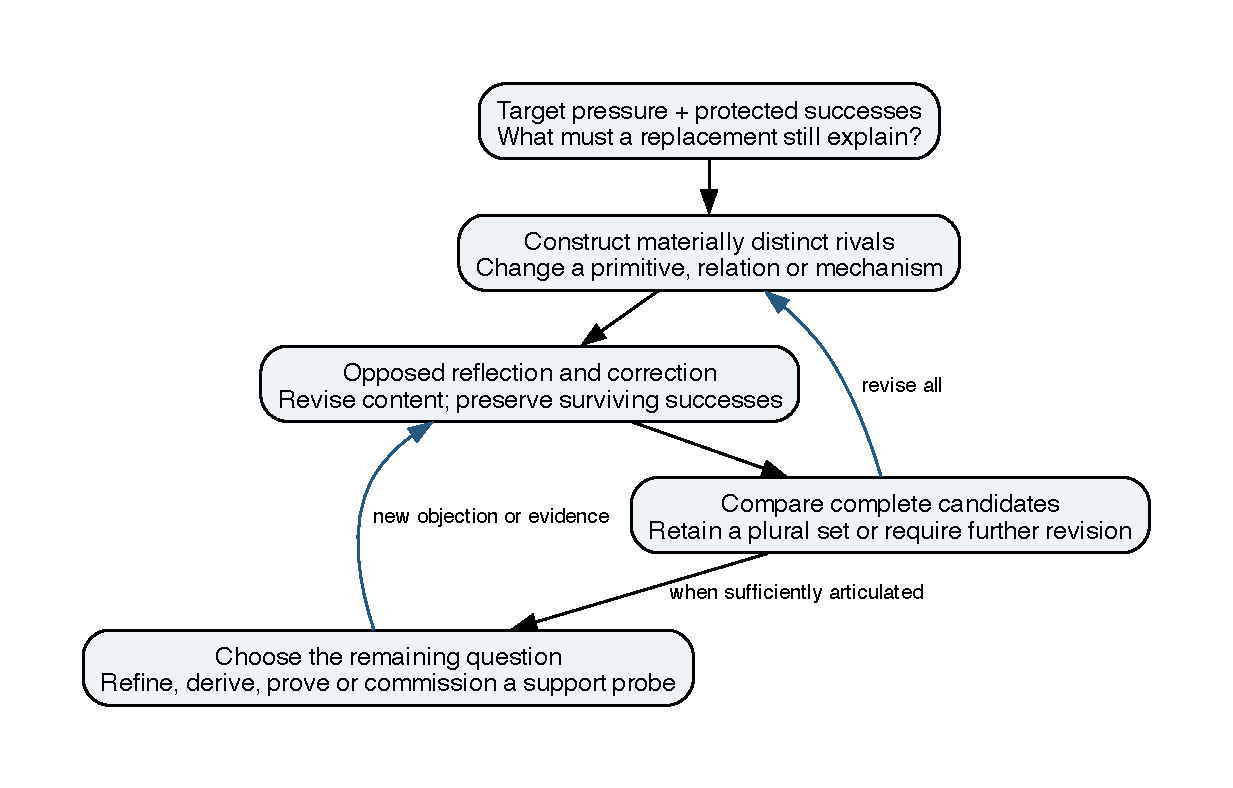
\includegraphics[width=.94\linewidth,height=.43\textheight,keepaspectratio]{paper-workflow-representations/mechanism-feedback.pdf}
\caption{The conceptual-invention branch of the underlying skill procedures; problems needing only ordinary derivation can bypass it. Criticism changes candidate content; comparison can retain a plural set; further work answers the remaining conceptual or evidential question. Feedback revises the relevant premise or representation. This is a skill-level account, not a claim that the native Prism projection implements every internal step or has been executed.}
\label{fig:mechanism-feedback}
\end{figure}
The workflow-specific accounts in Appendix~\ref{app:granular-prism-workflows} connect these mechanisms to their source instructions and contracts. A native projection hole marks an incomplete representation or realization at that boundary; it does not, by itself, mean that the repository contains no account of the conceptual work behind it.
